\part{Terminals}
\begin{frame}
\partpage
\end{frame}

\section{Terminal windows}
\begin{frame}{Terminal windows}
\begin{itemize}
\item Most of our work will be using the Linux terminal
\item The icon you click to start the terminal looks like this:

\includegraphics{imgs/terminal-icon.png}
\item The bar on the left hand side is called your 'Launcher'
\end{itemize}
\end{frame}

\section{The Launcher}
\begin{frame}{Section 1: The Launcher}
\begin{itemize}
\item Only a few applications are in your launcher
\item You can search for more applications i.e. gedit
\item Use the icon in the top left corner:
\begin{figure}[h]
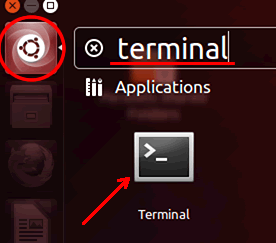
\includegraphics[height=0.3\textheight]{imgs/ubuntu-search-icon.png}
\end{figure}
\end{itemize}
\end{frame}

\section{Terminals on remote systems}
\begin{frame}{Section 1: Terminals on remote system}
\begin{itemize}
\item It is quite common to only have command line terminal access on a remote machine
\item I would assume most of you have Mac or Windows laptops
\item Mac users, OS X has a built in terminal
\item Windows users, you will need to install Putty to get a terminal client
\item We have put details about this in the notes
\end{itemize}
\end{frame}

\section{Text consoles}
\begin{frame}{Section 1: Text Consoles}
\begin{itemize}
\item Linux server administrators often dispense with the graphical environment entirely
\item One of the exercises involves starting a text based console
\item When you push the keys \begin{semiverbatim}[Ctrl]+[Alt]+[F2]\end{semiverbatim} your desktop will disappear!
\item It's not gone, you've just dropped down to a text based console
\item Remember that \begin{semiverbatim}[Ctrl]+[Alt]+[F7]\end{semiverbatim} returns you back to the graphical interface
\end{itemize}
\end{frame}

\section{Exercises}
\begin{frame}{Section 1: Exercises}
\begin{itemize}
\item In the notes go to Section 1: Terminal windows and text consoles
\item Read the notes for Section 1 
\item Attempt exercises 1 and 2
\item Raise your hand if you are stuck
\item We can demonstrate or explain an exercise
\end{itemize}
\end{frame}